%
% 03_konvexe_polygone.tex -- Einfuhrung in den Satz von Jordan fuer konvexe Polygone
%
% (c) 2026 Dominik Castelberg, Ostschweizer Fachhochschule
%
% !TEX root = ../../buch.tex
% !TEX encoding = UTF-8
%
\section{Der Fall konvexer Polygone
\label{jordan:section:konvexe_polygone}}
\kopfrechts{Der Fall konvexer Polygone}

Konvexe Polygone sind eine spezielle Art von Polygonen, welche selbst eine spezielle Form von einfach geschlossenen Kurven sind.

\begin{definition}[Polygon\label{jordan:definition:polygon}]
    Ein \emph{Polygon} ist eine geschlossene, stückweise lineare Kurve in der Ebene $\mathbb{R}^2$, die durch eine endliche Anzahl von Eckpunkten und Kanten, die diese Eckpunkte verbinden, definiert ist.
\index{Polygon}%
\end{definition}


Der Beweis des Satzes von Jordan für konvexe Polygone kann aus der Definition der konvexen Hülle als Schnittmenge aller Halbebenen, die alle Eckpunkte des Polygons enthalten, abgeleitet werden.

Halbebenen erlauben es uns, eine Ebene in zwei Gebiete zu unterteilen, die jeweils offen und wegzusammenhängend sind.

\begin{definition}[Halbebene\label{jordan:definition:halbebene}]
\index{Halbebene}%
    Eine \emph{Halbebene} in der Ebene $\mathbb{R}^2$ ist die Menge aller Punkte, die auf einer Seite einer Geraden liegen.

\end{definition}


Wenn man nun die Kanten eines konvexen Polygons zu Geraden gleicher Richtung verlängert, teilt jede dieser Geraden die Ebene in zwei Halbebenen.
Die Schnittmenge all dieser Halbebenen bildet die konvexe Hülle des Polygons, welche die Eigenschaften der Offenheit und des Wegzusammenhangs von den Halbebenen erbt.

\begin{definition}[Konvexe Hülle\label{jordan:definition:konvexe_huelle}]

    Die konvexe Hülle einer Menge von Punkten $S$ in der Ebene $\mathbb{R}^2$ ist die kleinste konvexe Menge, die alle Punkte in $S$ enthält.

    Die Schnittmenge aller Halbebenen, die alle Punkte in $S$ enthalten, bildet die konvexe Hülle von $S$.

\end{definition}

\begin{figure}
    \centering
    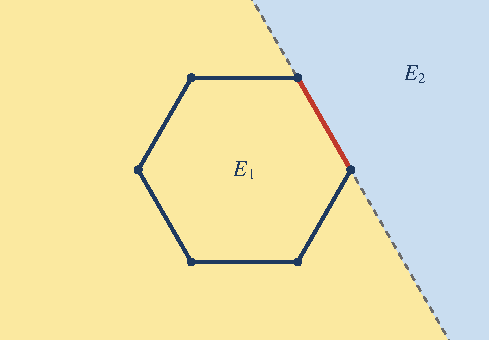
\includegraphics{papers/jordan/images/polygon_halbebene.pdf}
    \caption{Aufteilung der Ebene $E$ durch eine erweiterte Hexagonseite in zwei Halbebenen $E_1$ und $E_2$.}
\end{figure}

Der Beweis des Satzes von Jordan für konvexe Polygone ergibt sich zum Grossteil direkt aus den Eigenschaften der konvexen Hülle und ist daher relativ trivial.

\subsubsection{Offenheit und Wegzusammenhang von $I$ und $A$
\label{jordan:konvex:offenheit_wegzusammenhang}}

Offenheit und Wegzusammenhang von $I$ und $A$ ergeben sich wie erwähnt direkt aus der Konstruktion der konvexen Hülle.

\subsubsection{Beschränktheit von $I$
\label{jordan:konvex:beschraenktheit_innen}}

Die Beschränktheit von $I$ ergibt sich ebenfalls aus der Konstruktion der Hülle, da die konvexe Hülle als Schnittmenge von inneren Halbebenen entlang der Kanten einer geschlossenen Kurve, welche nur aus endlich vielen Kanten besteht, beschränkt sein muss.

\subsubsection{Unbeschränktheit von $A$
\label{jordan:konvex:unbeschraenktheit_aussen}}

Die Unbeschränktheit von $A$ ergibt sich aus der Tatsache, dass sowohl $I$ als auch $P$ beschränkt sind, und $A$ somit unbeschränkt sein muss, damit $I \cup P \cup A = \mathbb{R}^2$ gilt.

\subsubsection{Nicht-Leerheit von $I$
\label{jordan:konvex:nichtleerheit_innen}}

$I$ ist nicht leer, da der Schwerpunkt eines konvexen Polygons immer innerhalb des Polygons liegt und somit in $I$ enthalten sein muss.

\subsubsection{Nicht-Leerheit von $A$
\label{jordan:konvex:nichtleerheit_aussen}}

$A$ kann nicht leer sein, da die leere Menge beschränkt ist und $A$ unbeschränkt sein muss.

\subsubsection{$P$ als gemeinsamer Rand von $I$ und $A$
\label{jordan:konvex:gemeinsamer_rand}}

Der Beweis dafür, dass $P$ der gemeinsame Rand von $I$ und $A$ ist, wird in zwei Schritten durchgeführt.
Erst wird gezeigt, dass jeder Punkt auf $P$ ein Randpunkt von $I$ und $A$ ist, und dann wird gezeigt, dass kein Punkt auf dem Rand von $I$ und $A$ nicht auf der Jordan-Kurve liegt.

Für den ersten Schritt können wir eine Eigenschaft sämtlicher $p \in P$ verwenden: Da $p$ auf einer Kante eines konvexen Polygons liegt, liegt es auch auf einer Geraden, welche zum Zweck der Konstruktion der konvexen Hülle zur Trennung der Ebene in zwei Halbebenen verwendet wurde.
Entsprechend ist $p$ garantiert ein Randpunkt zu $A$, da für jede Gerade, die zur Konstruktion verwendet wurde, mindestens eine Halbebene existiert, die komplett in $A$ liegt.
Ob $p$ auch ein Randpunkt zu $I$ ist, können wir aus den Eigenschaften der konvexen Hülle als Schnittmenge aller inneren Halbebenen ableiten.
Damit ein $p$ ein Randpunkt zu $I$ ist, muss er sich in jeder abgeschlossenen inneren Halbebene befinden, aber gleichzeitig mindestens eine offene innere Halbebene verlassen.
Dies ist für alle $p \in P$ der Fall: Liegt $p$ auf einer Ecke, so verlässt er zwei offene innere Halbebenen, und liegt $p$ auf einer Kante, so verlässt er eine offene innere Halbebene.
Entsprechend ist $p$ garantiert ein Randpunkt zu $I$.

Für den zweiten Schritt nutzen wir die Offenheit von $I$ und $A$.
Da $I$ und $A$ offen sind und das Komplement von $P$ bilden, kann kein Punkt auf dem Rand von $I$ und $A$ nicht auf $P$ liegen.

\subsection{Der Satz von Jordan für konvexe Polygone
\label{jordan:subsection:satz_von_jordan_konvexe_polygone}}

Wir zeigen also auf, dass der Satz von Jordan für konvexe Polygone gilt.
Einfache geschlossene Kurven können jedoch auch nicht-konvexe Formen annehmen, was den Beweis für konvexe Polygone erneut unzureichend macht, um den Satz von Jordan im Allgemeinen zu beweisen.
